\section{Введение}
\label{sec:Chapter0} \index{Chapter0}

В данной главе вводятся базовые понятия, необходимые для постановки задачи.

\subsection{Компиляция}
\textbf{Компиляция} — это технология преобразования исходного кода, написанного на языке программирования высокого уровня (например, C, C++, Java), в машинный код или код, исполняемый целевой машиной.

Компиляция включает в себя несколько этапов:
\begin{enumerate}
    \item \textit{Лексический анализ (лексинг)}: Разбиение исходного кода на лексемы — минимальные синтаксически значимые единицы.
    \item \textit{Синтаксический анализ (парсинг)}: Проверка синтаксической правильности кода и его преобразование в дерево синтаксического разбора (AST).
    \item \textit{Семантический анализ}: Проверка корректности использования переменных, типов данных и других языковых конструкций.
    \item \textit{Генерация промежуточного кода}: Создание кода на промежуточном языке, который проще анализировать и оптимизировать.
    \item \textit{Оптимизация}: Улучшение промежуточного кода для повышения производительности и уменьшения размера.
    \item \textit{Генерация машинного кода}: Преобразование промежуточного кода в машинный код.
    \item \textit{Линковка (связывание)}: Объединение скомпилированных файлов и библиотек в один исполняемый файл.
\end{enumerate}

\textbf{Компилятор} — это программа, которая выполняет процесс компиляции. Она принимает исходный код и производит на его основе машинный код. Компиляторы могут быть разными для разных языков программирования и целевых платформ. Например, GCC (GNU Compiler Collection) — это компилятор для языков C, C++, и Fortran. %добавить ссылку на gcc

В данной работе основное внимание будет уделено пункту 5, а именно разработке алгоритма оптимизации на базе компилятора GCC. GCC является современным оптимизирующим компилятором, который широко используется в различных областях разработки программного обеспечения.

Основные виды компиляторов:
\begin{enumerate}
    \item \textit{Однопроходный компилятор}: Выполняет компиляцию за один проход, что обычно быстрее, но может ограничивать возможности оптимизации.
    \item \textit{Многопроходный компилятор}: Выполняет несколько проходов по исходному коду, позволяя более тщательно анализировать и оптимизировать код.
    \item \textit{Кросс-компилятор}: Компилирует код на одной платформе для выполнения на другой.
    \item \textit{Just-in-time (JIT) компилятор}: Компилирует код во время выполнения программы, улучшая производительность за счёт оптимизаций, которые невозможны при статической компиляции.
\end{enumerate}

Компиляторы играют важную роль в процессе разработки программного обеспечения, позволяя программистам писать код на высокоуровневых языках и затем преобразовывать его в эффективный исполняемый машинный код. Разработка оптимизаций для повышения производительности исполнения кода является основополагающей задачей в современных многопроходных компиляторах.

\subsection{Промежуточное представление программы}

\textbf{Промежуточное представление} (IR - Intermediate Representation) — это форма представления программы, используемая в компиляторах между этапами анализа исходного кода и генерации машинного кода. Оно играет важную роль в компиляции и позволяет упростить и улучшить процесс преобразования исходного кода в машинный код. Промежуточный код упрощает выполнение различных оптимизаций, поскольку он обычно более абстрактен, чем исходный код или машинный код.  На рис. ~\ref{flow} приводится структура
компилятора по Aho и др. \cite{aho2006compilers}

\begin{figure}[!htb]
    \centering
    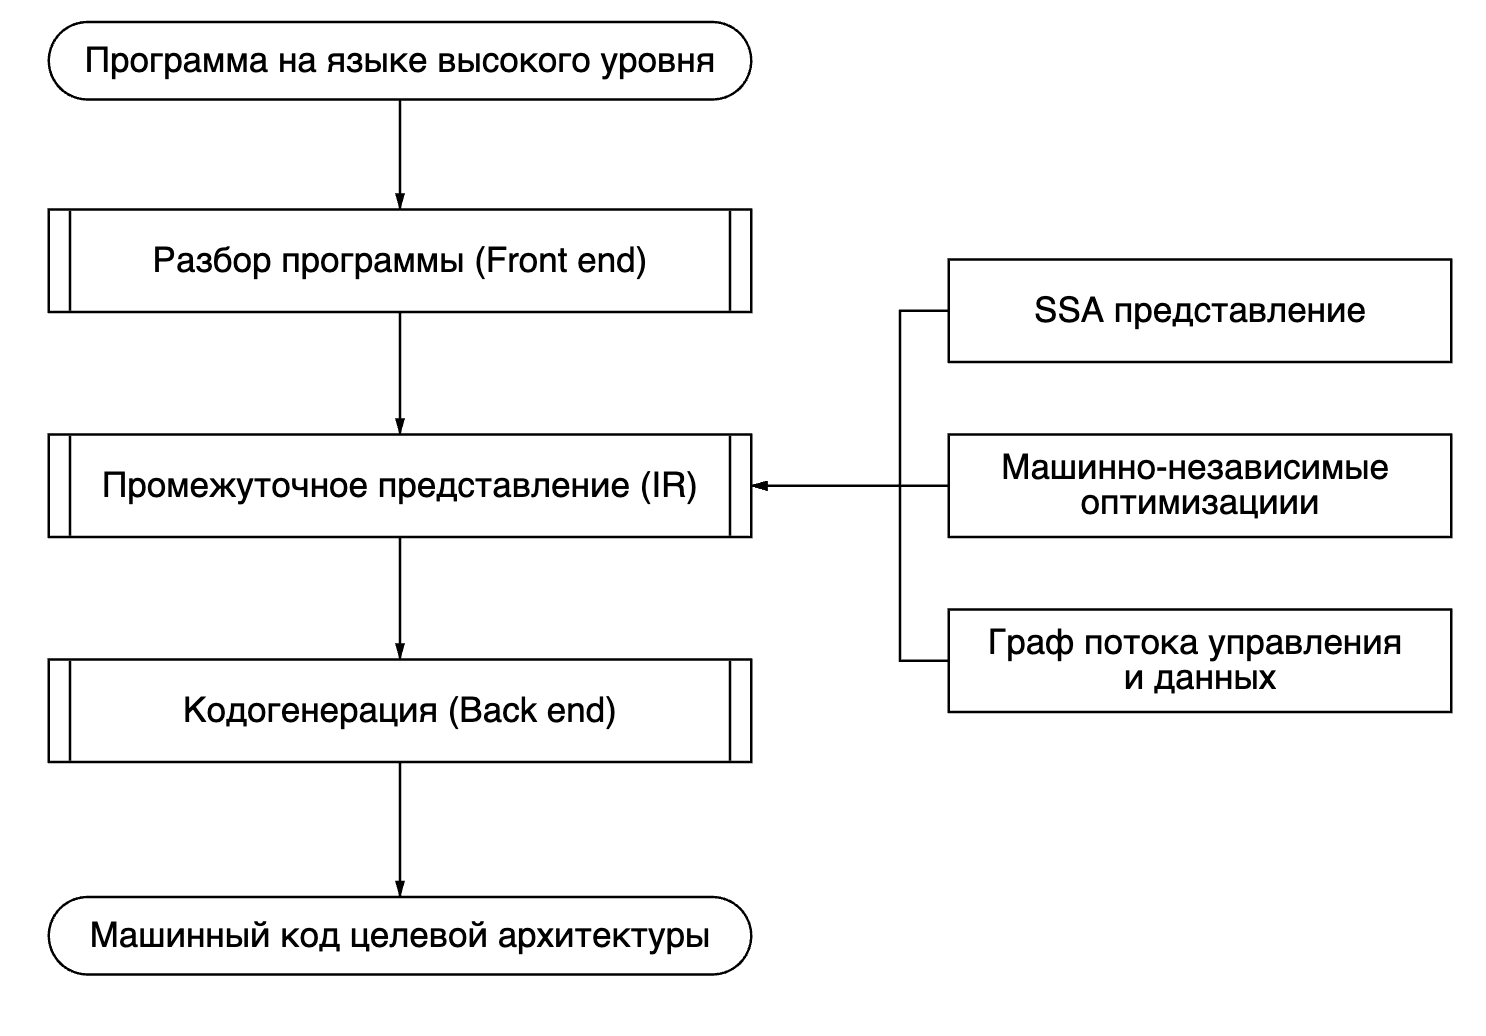
\includegraphics[scale=0.5]{compiler_flow.png}\\
    \caption{Структура компилятора}
    \label{flow}
\end{figure}

В GCC используются несколько видов промежуточных представлений, среди которых ключевыми являются GIMPLE и RTL:

\textit{GIMPLE} — это высокоуровневое промежуточное представление, используемое в GCC. Оно является упрощенной версией исходного кода, предназначенной для анализа и оптимизации. 

\textit{RTL} — это более низкоуровневое промежуточное представление, используемое в GCC для представления программы ближе к машинному коду.

GIMPLE используется в основном для машинно-независимых оптимизаций на более высоком уровне абстракции, таких как межпроцедурные оптимизации и преобразования графов потока управления и данных (более подробно рассмотрена в главе 1.2.2 и 1.2.3). RTL используется для оптимизаций, специфичных для целевой архитектуры, таких как распределение регистров и генерация инструкций. В данной работе для реализации алгоритма векторизации ленивых вычислений будет использоваться первый вид промежуточного представления.

Основные характеристики GIMPLE:
\begin{enumerate}
    \item \textit{Трехадресный код}: GIMPLE представляется в виде трехадресного кода, где каждая инструкция имеет не более трех операндов.
    \item \textit{Упрощение сложных выражений}: Сложные выражения разбиваются на более простые, что упрощает последующую обработку.
    \item \textit{SSA-форма (Static Single Assignment)}: GIMPLE преобразуется в SSA-форму, в которой каждая переменная присваивается единожды.
\end{enumerate}

\begin{figure}[!htb]
    \centering
    \includesvg[scale=1]{ctogimple.svg}
    \caption{Пример преобразования кода на С в GIMPLE}
\end{figure}

Введем понятия, относящиеся к промежуточному представлению программы. 

\subsubsection{Трехадресный код}
\textbf{Трехадресный код} (Three-Address Code, TAC) и его реализация в виде GIMPLE в компиляторе GCC представляет собой промежуточное представление, где каждая инструкция имеет не более трех операндов. Трехадресный код состоит из инструкций, каждая из которых может быть представлена в следующем общем виде:

\begin{equation}
    (res, op, x, y)
\end{equation}

где
\begin{itemize}
    \item $op$ - код оператора(операции)
    \item $x$ и $y$ - аргументы, подающиеся на вход оператора
    \item $res$ - результат, вырабатываемый оператором(операцией)
\end{itemize}

Например, \textit{присваивание} в SSA-форме (более подробно рассмотрено в главе 1.2.4) будет иметь следующий вид:

\begin{equation}
    res = (op, x, y)
    \label{formula assign}
\end{equation}

Следует учесть, что некоторые операторы могут иметь только один аргумент или не иметь их вовсе, тогда соответствующие элементы оставляются пустыми.

\subsubsection{Граф потока управления}

\textbf{Граф потока управления} (Control Flow Graph, CFG) является важным инструментом в компиляторах, включая такие, как GCC (GNU Compiler Collection). Он используется для представления возможных путей выполнения программы и помогает оптимизировать и анализировать код.

CFG состоит из следующих основных компонентов:

\begin{itemize}
    \item \textit{Узлы (Nodes)}: Каждый узел представляет собой базовый блок (basic block) — последовательность инструкций, выполняемых последовательно без переходов.
    \item \textit{Дуги (Edges)}: Дуги соединяют узлы и обозначают возможные переходы управления между ними. Они могут быть условными (в случае ветвлений) и безусловными (например, вызовы функций или переходы).
\end{itemize}

Прежде чем дать определение базового блока, следует сказать, что операции по их влиянию на ход исполнение программы относят к двум видам: изменяющие ход исполнения и не изменяющие. Первые это обычно операторы условного или безусловного перехода, а также вызова функций. Главное свойство этих операторов - изменение линейного потока управления программы. Вторые это операторы, результат выполнения которых никак не влияет на линейное исполнение программы.

\textit{Базовым блоком} назовем совокупность операций, не изменяющих ход исполнения программы со следующими свойствами:
\begin{enumerate}
    \item Управление базовому блоку может передаваться только через первую инструкцию блока.
    \item Управление передается от базового блока только через последнюю инструкцию блока
\end{enumerate}

Соответственно, передачи управления от одного базового блока к другому — \textit{дугами} графа. На основании анализа CFG компилятор может проводить различные оптимизации, такие как удаление мертвого кода, инлайнинг функций, развертку циклов и другие.

\subsubsection{Граф потока данных}

\textbf{Граф потока данных} (Data Flow Graph, DFG) — это структурное представление программ, которое используется для анализа потоков данных в компиляторах. В отличие от графа потока управления (CFG), который фокусируется на последовательности выполнения команд, DFG концентрируется на зависимости данных между различными частями программы.

DFG состоит из следующих компонентов:

\begin{itemize}
    \item \textit{Узлы (Nodes)}: Каждый узел представляет собой операцию или вычисление, выполняемое в программе, например, арифметическую операцию или присваивание.
    \item \textit{Рёбра (Edges)}: Рёбра обозначают потоки данных между узлами. Они показывают, как результаты одной операции используются в качестве входных данных для другой.
\end{itemize}

DFG позволяет выявлять независимые операции, которые могут быть выполнены параллельно. Это особенно важно для современных многоядерных процессоров и архитектур с поддержкой параллельных вычислений. Также DFG позволяет проводить так называемый \textit{def-use} анализ, который в дальнейшем будет использоваться в данной работе.

\textbf{Def-use анализ} (анализ определения и использования) — это метод анализа данных, используемый в компиляторах для отслеживания, где в программе значения переменных определяются (присваиваются) и где они затем используются (читаются).

Процесс \textit{def-use} анализа выглядит следующим образом.
\begin{enumerate}
    \item \textit{Выявление определений и использований}:
        \begin{itemize}
            \item Определения (\textit{def}) — это инструкции, которые присваивают значение переменной (например, $x$ = 5;)
            \item Использования (\textit{use}) — это инструкции, которые читают значение переменной (например, $y$ = $x$ + 1;)
        \end{itemize}
    \item \textit{Построение def-use цепочек}:

    Def-use цепочка связывает каждое определение переменной с ее использованными значениями. Например, если переменная $x$ определяется в одной инструкции и используется в нескольких других, создается связь между этими инструкциями.
    \item \textit{Анализ потоков управления:}
    
    Для корректного анализа def-use необходимо учитывать возможные пути выполнения программы. Это обычно делается с помощью графа потока управления (CFG), где для каждого базового блока анализируются определения и использования переменных.
\end{enumerate}

В компиляторах, таких как GCC, оба графа могут использоваться совместно для комплексного анализа программ. На основе CFG можно построить DFG для каждого базового блока, чтобы детально проанализировать потоки данных внутри блока. Информация из DFG может быть использована для улучшения глобальных оптимизаций на уровне CFG, таких как перемещение инвариантов цикла или оптимизация ветвлений.

\subsubsection{SSA-представление}

\textbf{Статическое однократное присваивание} (Static Single Assignment, SSA) — это форма промежуточного представления программы, используемая в компиляторах для упрощения анализа и оптимизации кода \cite{cytron1991efficiently}. В SSA каждая переменная присваивается только один раз, а все использованные переменные явно указывают на свое определение. Это достигается путем введения новых переменных при каждом присваивании.

Основные понятия SSA:
\begin{itemize}
    \item \textit{Присваивание}: Каждое присваивание переменной получает уникальное имя, что устраняет неоднозначность в определении переменных.
    \item \textit{Функции $\varphi$ (phi)}: Используются для объединения значений переменных из различных путей потока управления. Эти функции помогают сохранить единственное присваивание переменной, даже если она может принимать разные значения в зависимости от пути выполнения программы.
\end{itemize}

\begin{figure}[!htb]
    \centering
    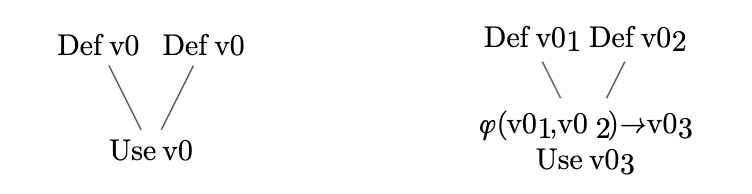
\includegraphics[scale=0.9]{ssa.png}
    \caption{Пример SSA-формы}
\end{figure}

Чтобы перевести код в форму статического единственного присваивания, всем объектам, хранящим в себе результат какой-либо операции, присваивается индивидуальный номер. В точках схождения нескольких определений для одного объекта вводится специальная операция - $\varphi$-функция, которая по своей сути объединяет два определения одного объекта в один, так как при реальном исполнении  произойдет только одно из определений.

\subsubsection{Ленивые вычисления}

\textbf{Ленивые вычисления}, также известные как {отложенные вычисления (lazy evaluation)}, это техника оптимизации, при которой вычисление выражения откладывается до тех пор, пока его значение действительно не понадобится. В языках программирования C и C++ ленивые вычисления поддерживаются через различные механизмы, стандартизованные самим языком.

\begin{figure}[!htb]
    \centering
    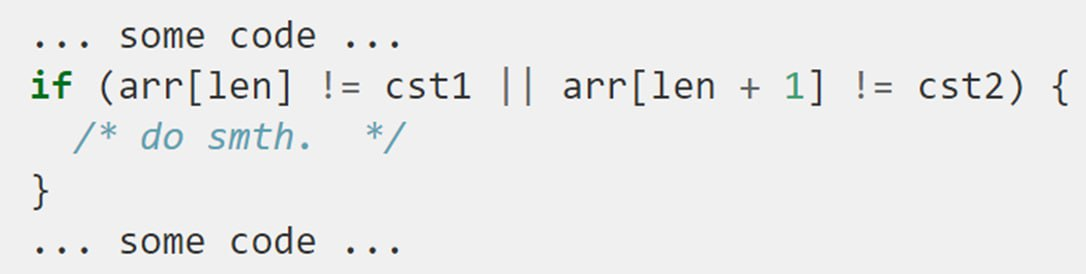
\includegraphics[scale=0.7]{lazyeval.jpg}
    \caption{Пример ленивых вычислений}
    \label{lazyeval}
\end{figure}

В C и C++ логические операторы $\&\&$ (логическое И) и $||$ (логическое ИЛИ) реализованы с использованием механизма \textit{краткого замыкания (Short-Circuit Evaluation)}. Это означает, что вычисление второго операнда происходит только в том случае, если значение первого операнда недостаточно для определения результата выражения. Общее назначение ленивых вычислений заключается в экономии времени на проведении вычислений, результаты которых заведомо не будут использованы программой в дальнейшем. Соответственно, за счет снижения объемов вычислений повышается производительность. 

\subsubsection{Product-Sum Form (PSF)}

\textbf{Product-Sum Form (PSF)} представляет из себя сумму произведений. Каждое произведение содер­жит в себе последовательность объектов, которые должны быть перемножены, а также постоянный множитель. Помимо произведений, сумма, по аналогии с первыми, имеет константное слагаемое.
В общем случае, PSF имеет следующий вид:

\begin{equation}
    PSF = c +\sum_{i}(p_i\cdot \prod_{k}x_{ik}),
\end{equation}

где $x_{ik}$ — перемножаемые объекты $i$-го слагаемого, $p_i$ — его константный множи­тель, $c$ — константное слагаемое всей формы.

PSF-формы могут быть использованы для проведения оптимизаций над выражениями, а также для анализа зависимостей данных.


\subsection{Векторизация}

\textbf{Векторизация} — это процесс преобразования обычного (скалярного) кода в код, который может выполняться на векторных или SIMD (Single Instruction, Multiple Data) процессорах. Основная цель векторизации — увеличить производительность программ за счёт параллельного выполнения одной и той же операции над несколькими данными одновременно.

\subsubsection{Методы векторизации}
Методы векторизации, представленные в современных компиляторах, обычно делятся на циклическую векторизацию и векторизацию линейного кода. Более подробно это будет рассмотрено в 3 главе. Сам же процесс векторизации выглядит примерно следующим образом:

\begin{enumerate}
    \item \textit{Анализ кода}: Компилятор анализирует исходный код программы для поиска циклов и других конструкций, которые могут быть векторизованы. Это часто означает поиск независимых операций, которые можно выполнять параллельно.
    \item \textit{Преобразование кода}: Обнаружив подходящие конструкции, компилятор преобразует их в векторные инструкции. Например, если в цикле происходит сложение элементов двух массивов, компилятор может заменить этот цикл одной или несколькими векторными инструкциями, которые выполняют это сложение над несколькими элементами массивов одновременно.
    \item \textit{Генерация векторных инструкций}: Компилятор генерирует соответствующие векторные инструкции для целевой архитектуры процессора. Различные процессоры поддерживают разные наборы векторных инструкций, такие как SSE, AVX для процессоров Intel, NEON для ARM и другие.
\end{enumerate}

\subsubsection{Таксономия Флинна}
По признаку наличия параллелизма в потоках данных и инструкций Майклом Флинном в 1996 году была предложена следующая классификация \cite{skillicorn1988taxonomy}:
\begin{itemize}
  \item \textbf{ОКОД(SISD) - } Система с одиночными потоками команд и данный (single instruction, single data). В данном классе отсутствует какой-либо параллелизм. Такая система исполняет инструкции последовательно, работая только с одним потоком данных.
  
  \item \textbf{ОКМД(SIMD) - } Система с одиночным потоком команд и множественным потоком данных (single instruction, multiple data). Машины этого класса загружают набор данных и одну инструкцию для исполнения. Этот класс является особенно важным для данной работу и будет описан детальнее в следующей главе.
  
  \item  \textbf{МКОД(MISD) -} Система с множественным потоком команд и одиночным потоком данных (multiple instruction, single data). Отказоустойчивый тип архитектуры, не получивший широкого распространения.
  
  \item  \textbf{МКМД(MIMD) -} Система с множественными потоками данных и команд (multiple instruction,multiple data). К этому классу обычно относят многопроцессорные системы и компьютерные кластеры. 
\end{itemize}

Важным для работы большинства векторизаторов является принцип SIMD. SIMD инструкции появились в процессорах еще 1990-x годах. С тех пор векторные расширения совершенствовались и на сегодняшний день существуют расширения с поддержкой инструкций длинной более 256 бит.

\newpage
